\subsection{Applikationserver [Team]}
\begin{wrapfigure}{r}{0.3\textwidth}
    \begin{center}
      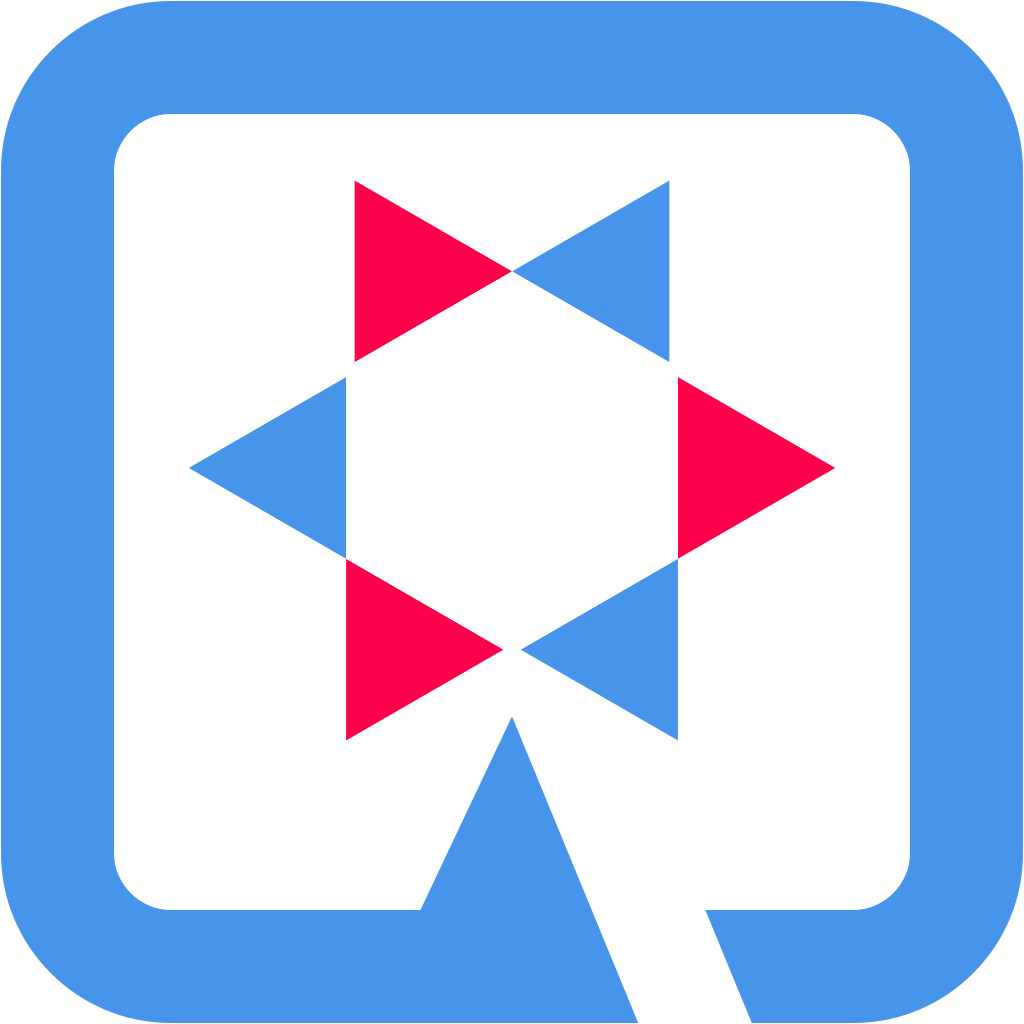
\includegraphics[width=0.2\textwidth]{pics/quarkus_logo.png}
     \caption{Quarkus Logo}
    \end{center}
  \end{wrapfigure}
Als Applikationsserver wurde \emph{Quarkus} ausgewählt. Quarkus zeichnen sich  durch kurze Startzeiten und gute Performance in Hinsicht auf den Verbrauch des Arbeitsspeichers aus. Nach der Erstellung eines neuen Projekts wird standardmäßig eine Maven-Struktur mitgeliefert. Zusätzlich verfügt Quarkus über eine Vielzahl von Extensions, welche durch CMD-Befehl oder manuell zu Projekten hinzugefügt werden können. \cite{QuarkusAbout, QuarkusFirstApplication}
Quarkus besitzt die Fähigkeit im Hintergrund nach jeder Änderung des Ausgangscodes die betroffenen Applikationen upzudaten und Unit-Tests auszuführen.
Die Services werden als REST-Services bereitgestellt. Quarkus besitzt eine einfache Konfigurationsmöglichkeit um REST-Services anzubinden. 

\subsection{Datenhaltung [Team]}
\begin{wrapfigure}{r}{0.3\textwidth}
    \begin{center}
      
\includegraphics[width=0.2\textwidth]{pics/postgres_logo.png}
     \caption{PostgreSQL Logo}
    \end{center}
  \end{wrapfigure}
PostgreSQL ist ein Open Source Managementsystem für relationale Datenbanken, welches seit 35 Jahren entwickelt wird. Hinter diesem System befindet sich eine große Community, welche weiterhin Features konstruieren. \cite{PostgreSQLAbout}






%%\section{Grundkriterien für das Backend [E]}
%%\setauthor{Halilovic Ema}
%%Die Grundkriterien für die Wahl der Tools und Technologien hier waren, dass diese fortlaufend weiterentwickelt werden 
%%und zum derzeitigen Standpunkt ein ausreichendes Spektrum an Funktionalität für Mikroservice-Architekturen ermöglichen.\cite{MicroserviceAbout} 
%%Ebenso sollen diese gute Dokumentationen und breite Communities enthalten. Schon vorhandene Praxiserfahrung stellte sich bei der finalen Auswahl als entscheidender Faktor dar.
%%
%%
%%
%%\section{PostgreSQL [E]}
%%\setauthor{Halilovic Ema}
%%PostgreSQL ist ein open source Managementsystem für relationale Datenbanken, welches seit 35 Jahren entwickelt wird. 
%%Hinter diesem System befindet sich eine große Community, welche weiterhin Features entwickelt. 
%%Die Entscheidung  Eine gute Dokumentation und die vielen verschiedenen Anwendungsfälle 
%%\cite{PostgreSQLAbout}
%%
%%\section{Quarkus [E]}
%%\setauthor{Halilovic Ema}
%%Unter Quarkus versteht man ein open source Framework, womit cloud-native Projekte in Java entwickeln werden können. 
%%Dieses zeichnen sich aus durch kurze Startzeiten und gute Performance in Hinsicht auf den Verbrauch des Arbeitsspeichers. 
%%Nach der Erstellung eines neuen Projekts wird standardmäßig eine \hyperref[ch::MavenTool]{Maven}-Struktur mitgeliefert.
%%Zusätzlich verfügt es eine Vielzahl von Extensions, welche durch Command-line-Befehle oder händisch zu Projekten hinzugefügt werden können.
%%
%%\cite{QuarkusAbout, QuarkusFirstApplication}
%%
%%\subsection{Maven [E]}
%%\label{ch::MavenTool}
%%\setauthor{Halilovic Ema}
%%Maven ist ein Tool, um den Kompilierungsprozess eines Projekts zu vereinfachen. 
%%Wenn man Projekte auf unterschiedlichen Geräten ausführen möchte kommt es dabei oftmals zu Problemen. Meist sind lokale Konfigurationen der Auslöser dafür.
%%Maven ermöglicht ebenso ein einheitliches System für Projektkonfigurationen, sodass diese nicht mehrmanuell bei Gerätewechsel umgestellt werden müssen. 
%%Dabei wird die \emph{pom.xml} Datei verwendet, welche eine der Hauptkomponenten ist für Maven-Projekte.
%%\cite{MavenAbout}
%%
%%In Quarkus-Projekten werden darin relevante Informationen gespeichert, wie zum Beispiel die verwendete Java Version oder alle verwendeten Extensions.
%%\
%%
%%\subsection{JDBC Driver - PostgreSQL [E]}
%%\setauthor{Halilovic Ema}
%%JDBC Driver - PostgreSQL ist eine Extenstion für Quarkus Projekte, die Datenbankverbindungen zu PostgreSQL Datenbanken ermöglicht.
%%Java JDBC gibt es als API für Java Anwendungen, jedoch unterschiedet diese sich von dem in Quarkus benutzten JDBC Driver.
%%
%%// TODO alles umschreben
%%Das JDBC steht für \emph{Java Database Connectivity} und .
%%
%%Um eine Datenbankverbindung aufzubauen muss man in die Datei \emph{application.properties} einige zusätzlichen Konfigurationen einfügen, wie den Pfad der Datenbank, die Art der Datenbank, den Nutzernamen und das Passwort \ref{lst:quarkusDatasource}:
%%
%%\begin{lstlisting}[caption=Beispielkonfigurationen,label=lst:quarkusDatasource]
%%  quarkus.datasource.db-kind=postgresql 
%%  quarkus.datasource.username=meinUser
%%  quarkus.datasource.password=meinPassword
%%  quarkus.datasource.jdbc.url=jdbc:postgresql://localhost:5432/meineDatabase
%%\end{lstlisting}
%%
%%\subsection{Hibernate ORM [E]}
%%\setauthor{Halilovic Ema}
%%// TODO
%%
%%\subsection{REST-Easy [E]}
%%\setauthor{Halilovic Ema}
%%REST-Easy ist eine Erweiterung für Quarkus, die es ermöglicht, im Quarkus Projekt mit Jakarta RESTful Web Servies zu arbeiten. 
%%
%%
%% \section{IntelliJ IDEA [E]}
%% \setauthor{Halilovic Ema}
%% IntelliJ IDEA ist eine IDE, welche von JetBrains entwickelt wurde. Diese ist ausgelegt für Java- und Kotlin-Projekte. 
%% Durch eingebaute Features erleichtert diese Entwicklungsumgebung das Programmieren für den*die Nutzer*in. 
%% Plug-Ins ermöglichen es, Datenbankverbindungen und weiteres in der IDE zu konfigurieren, sodass dem*der Entwickler*in eine Übersicht von benötigten Informationen gegeben werden kann.
%% \cite{IntelliJIDEA}
%%
%%\section{Oracle Server [E]}
%%\setauthor{Halilovic Ema}
%%// TODO